\documentclass{article}
\renewcommand{\baselinestretch}{1.25} 
\usepackage[table]{xcolor}
\usepackage[margin=0.5in]{geometry}
\usepackage{longtable}
\usepackage{graphicx}
\usepackage{enumitem}
\usepackage{booktabs}
\usepackage{float}
\usepackage{caption}
\usepackage{subcaption}

\begin{document}

\title{Standard Operating Procedure}
\date{\today}
\author{Synthesizing Polymer Films via Slip-Coat Technique}

\maketitle

\begin{center}
\begin{tabular}{ |c|c| }
\hline
\cellcolor{gray!25} Procedure Title & Slip-Coating of Polymer Films \\
\hline
\cellcolor{gray!25} Procedure Author & Matteo Fulghieri, Trevor Wiechmann \\
\hline
\cellcolor{gray!25} Supervisor & Amy Cordones-Hahn \\
\hline
\cellcolor{gray!25} Location & Bldg. 40, Rm. 128 \\
\hline
\end{tabular}
\end{center}

\begin{center}
\begin{tabular}{ |p{\textwidth}| }
\hline
\cellcolor{gray!25} \#1 \textbf{Procedural Description} \\
\hline
This procedure details the synthesis of polymer thin films using a slip-coating technique, and it explains necessary safety precautions associated with the procedure. Batches of 10-20 films are made in 1-2 hours. Films may be used immediately or stored. \\  
\hline
\end{tabular}
\end{center}

\begin{center}
\begin{tabular}{ |p{\textwidth}| }
\hline
\cellcolor{gray!25} \#2 \textbf{Risk Assessment} \\
\hline
a) \underline{Chemical Exposure:} Common chemicals used to dissolve the polymers (such as acetone, chloroform, cyclohexanone, dichloromethane, dimethyl sulfoxide, and tetrahydrofuran) pose health risks of varying severities. These risks include acute risks (irritation) and chronic risks (cancer, organ damage, and nervous system damage). Safety precautions (see next section) then pertain to limiting exposure. \\
b) \underline{Flammability}: In addition to chemical exposure, solvents also pose a flammability hazard. Safety precautions then pertain to minimizing fire risk and peroxide formation. \\
c) \underline{Puncture/Sharp Hazards}: This procedure uses both glass slides and syringes. Broken glass slides and unsealed syringes pose physical hazards via puncture wounds (``needlestick") or exposure to glass shards. \\ 
d) \underline{Pressurized Gases}: This procedure may require the use of peroxide-forming solvents. Extracting such solvents requires use of pressurized gases. \\
\hline
\end{tabular}
\end{center}

\begin{center}
\begin{longtable}{ |p{\textwidth}| }
\hline
\cellcolor{gray!25} \#3 \textbf{Safety Procedures} \\
\hline
a) \underline{Fire/Explosion Protection}: Correct storage of flammable solvents is strictly necessary. Solvents such as cyclohexanone and tetrahydrofuran must be stored in air-impermeable containers as to prevent the formation of peroxides. Extraction of the solvent similarly requires proper technique. An SOP for peroxide forming chemicals should be referred to. Furthermore, proper storage of flammable solvents requires use of a fire cabinet. \\
b) \underline{Personal Protective Equipment}: Correct PPE includes eye protection, gloves, and long sleeves/pants. Correct PPE minimizes skin contact with potentially harmful solvents and offers some protection to sharps such as broken glass. \\
c) \underline{Puncture/Sharp Protection}: Sharps must be properly handled to avoid injury. Syringes should be uncapped using the same hand which holds the syringe. That is, the syringe is held between the palm and three lateral fingers. The index finger and thumb is used to remove the cap. Further, care must be taken to not break glass slides; however, small chips may be difficult to avoid. Thus, chips should be taken note of and the slide properly disposed of. \\
d) \underline{Ventillation Control}: Uncovered solvents/solutions must be operated only within the fume hood, thereby reducing exposure to aerosolized/vaporized solvents. \\
\begin{center}
	\textit{Continued from last page...}
\end{center}
e) \underline{Accessible Safety Equipment}:
\begin{enumerate}
	\item \textbf{Chemical Spill Kits} are located above the fire cabinet. If a chemical spill poses an immediate health or environment emergency, then 911 must be contacted. If not, a chemical spill should be reported to ext. 5555. 
	\item \textbf{Fire Alarm Manual Pull Handle} is located outside the lab, near the building exit.
	\item \textbf{Fire Extinguisher} is located immediately outside of the lab to the right-hand side if exiting the lab.
	\item \textbf{First Aid Kits} are located above the fire cabinet. Life threatening injuries must be reported first to 911, then to ext. 5555, then to the supervisor. Non-life threatening injuries must be reported first to the supervisor and then to either SLAC Medical or ext. 5555. ``If in doubt, call 911 or ext. 5555."
	\item \textbf{Fumehoods} are located along the left-hand wall after entering the lab.
	\item \textbf{Personal Protection Equipment} is located to the left-hand side of the door if entering the lab.
	\item \textbf{Shower and Eye Washing Station} are located to the right-hand side of the door if entering the lab.
	\item \textbf{Telephone} is located adjacent to lab entrance.
\end{enumerate}
\\  
\hline      
\end{longtable}
\end{center}

\begin{center}
\begin{tabular}{ |p{\textwidth}| }
\hline
\cellcolor{gray!25} \#4 \textbf{Designated Area} \\
\hline
Fume hood 1 or 2, in Room 128 of Building 40. \\ 
\hline
\end{tabular}
\end{center}


\begin{center}
\begin{longtable}{ |p{\textwidth}| }
\hline
\cellcolor{gray!25} \#5 \textbf{Step-By-Step Operating Procedure} \\
\hline
This section is split into four distinct subsections: preparing solutions, preparing films, measuring film thickness, and cleaning. \\
\textbf{Equipment}
\begin{enumerate}[series=TF]
	\item \textit{Preparing Solutions}
	\begin{itemize}
		\item 10 mL syringe
		\item 20 mL scintillation vials
		\item Electronic balance
		\item Polymers (e.g. PVC, PS, PMMA)
		\begin{itemize}
			\item Note: Polymers have varying usability. For example, PMMA was a fine powder while PS had distinct spherical units.
		\end{itemize}
		\item Solvents (e.g. acetone, cyclohexane, DCM, DSMO, THF)
		\item Scoopula 
		\item Sonicator
	\end{itemize}
\end{enumerate}
\begin{center}
	\textit{Continued on next page...}
\end{center}
\\
\begin{enumerate}[resume*=TF]
	\item \textit{Preparing Films}
	\begin{itemize}
		\item 1 mL syringe
		\item Frosted Scotch tape
		\item VMR VistaVision microscope slides
	\end{itemize}
\end{enumerate}
\begin{enumerate}[resume*=TF]
	\item \textit{Measuring Film Thickness}
	\begin{itemize}
		\item FTIR mounts
		\item UV-vis Spectrophotometer (Cary 50)
	\end{itemize}
\end{enumerate}
\begin{enumerate}[resume*=TF]
	\item \textit{Cleaning}
	\begin{itemize}
		\item Acetone
		\item Isopropanol
		\item KimWipes or lens wipes
		\item Sonicator
	\end{itemize}
\end{enumerate}
\\
\textbf{Procedure}
\begin{enumerate}[series=TE]
	\item \textit{Preparing Solutions} ($\approx$ 1.5 wt\%)
	\begin{itemize}
		\item Note: This solvent procedures are conducted within the fume hood.
	\end{itemize} 
	\begin{enumerate}
		\item Prepare a scintillation vial by uncapping and taring it.
		\item Using the scoopula, add solid polymer ($\approx$ 70 mg).
		\item Use 1 mL and 10 mL syringes to add desired amount of each solvent to vial ($\approx$ 5 mL).
		\item Label vial with contents and initials of responsible person.
		\item Sonicate vial for 90 minutes with heat applied.
	\end{enumerate}
	\begin{itemize}
		\item Notes: 
		\begin{itemize}
			\item One 5 mL vial can make up to 200 films.
			\item Batch size may be 10 vials containing 0.1 wt\% increments from 1.1 to 2.0 wt\%.
		\end{itemize}  
	\end{itemize}
\end{enumerate}
\begin{center}
	\textit{Continued on next page...}
\end{center}
\\
\begin{enumerate}[resume*=TE]
	\item \textit{Preparing Films}
	\begin{enumerate}
		\item Acquire two clean microscope slides, placing one slide in the hand and the other somewhere accessible.
		\item Using a 1 mL syringe, deposit $\approx$ 50 \textmu L of polymer solution onto the slide held in the hand (see figures after section).
		\item Set the syringe down, and place the second slide on top of the first, squeezing the solution between the two slides.
		\begin{itemize}
			\item Cover $\approx$ 3/4-ths of the slide.
			\item Confirm there are no air bubbles or irregularities between the slides.
		\end{itemize}
		\item Swiftly pull the two slides apart.
		\item Place the two slides down with the coated side facing up.
		\item Allow to dry for at least 60 seconds, optionally followed by 10 seconds of heat applied from more than a foot away.
		\item Once dry, construct a tape frame from the Scotch tape.
		\begin{itemize}
			\item Apply the tape in a clockwise or counterclockwise direction, beginning with the long edge.
			\item Do not allow the tape to touch the glass slide directly; instead, have it contact only the polymer coating.
		\end{itemize}
		\item Affix a long edge of tape to a straight edge such as a table (see figures after section).
		\item Delaminate using a circular motion corresponding to the order the tape was applied.
		\item Remove framed film from the straight edge.
	\end{enumerate}
\end{enumerate}
\begin{enumerate}[resume*=TE]
	\item \textit{Measuring Thickness}
	\begin{enumerate}
		\item Using the film framed in tape, apply to a FTIR mount (see figures after section).
		\begin{itemize}
			\item Make sure to align over the correct height of the spectrophotometer beam.
			\item As often as possible, pull from the short edge so that strain is put on the long edges of tape.
		\end{itemize}
		\item After preparing the spectrophotometer to scan, begin by scanning a blank (i.e. no film in apparatus).
		\item Place the mounted film into the UV-vis spectrophotometer.
		\item Scan the film at several locations.
		\item By exporting the data as a CSV file, the associated programs will determine film thickness.
	\end{enumerate}
\end{enumerate}
\begin{enumerate}[resume*=TE]
	\item \textit{Cleaning (and Managing Waste)}
	\begin{enumerate}
		\item Place dirty slides into a 250 mL jar with acetone
		\item Seal jar, and place into sonicator for 30 minutes with heat applied
		\item Remove from sonicator and wipe down with isopropanol
		\begin{itemize}
			\item Using a lens wipe leaves behind significantly less residue than using a KimWipe
		\end{itemize}
	\end{enumerate}
\end{enumerate}
\\ \hline
\end{longtable}
\end{center}

\begin{figure}[H]
	\centering
	\captionsetup{width=14cm}
	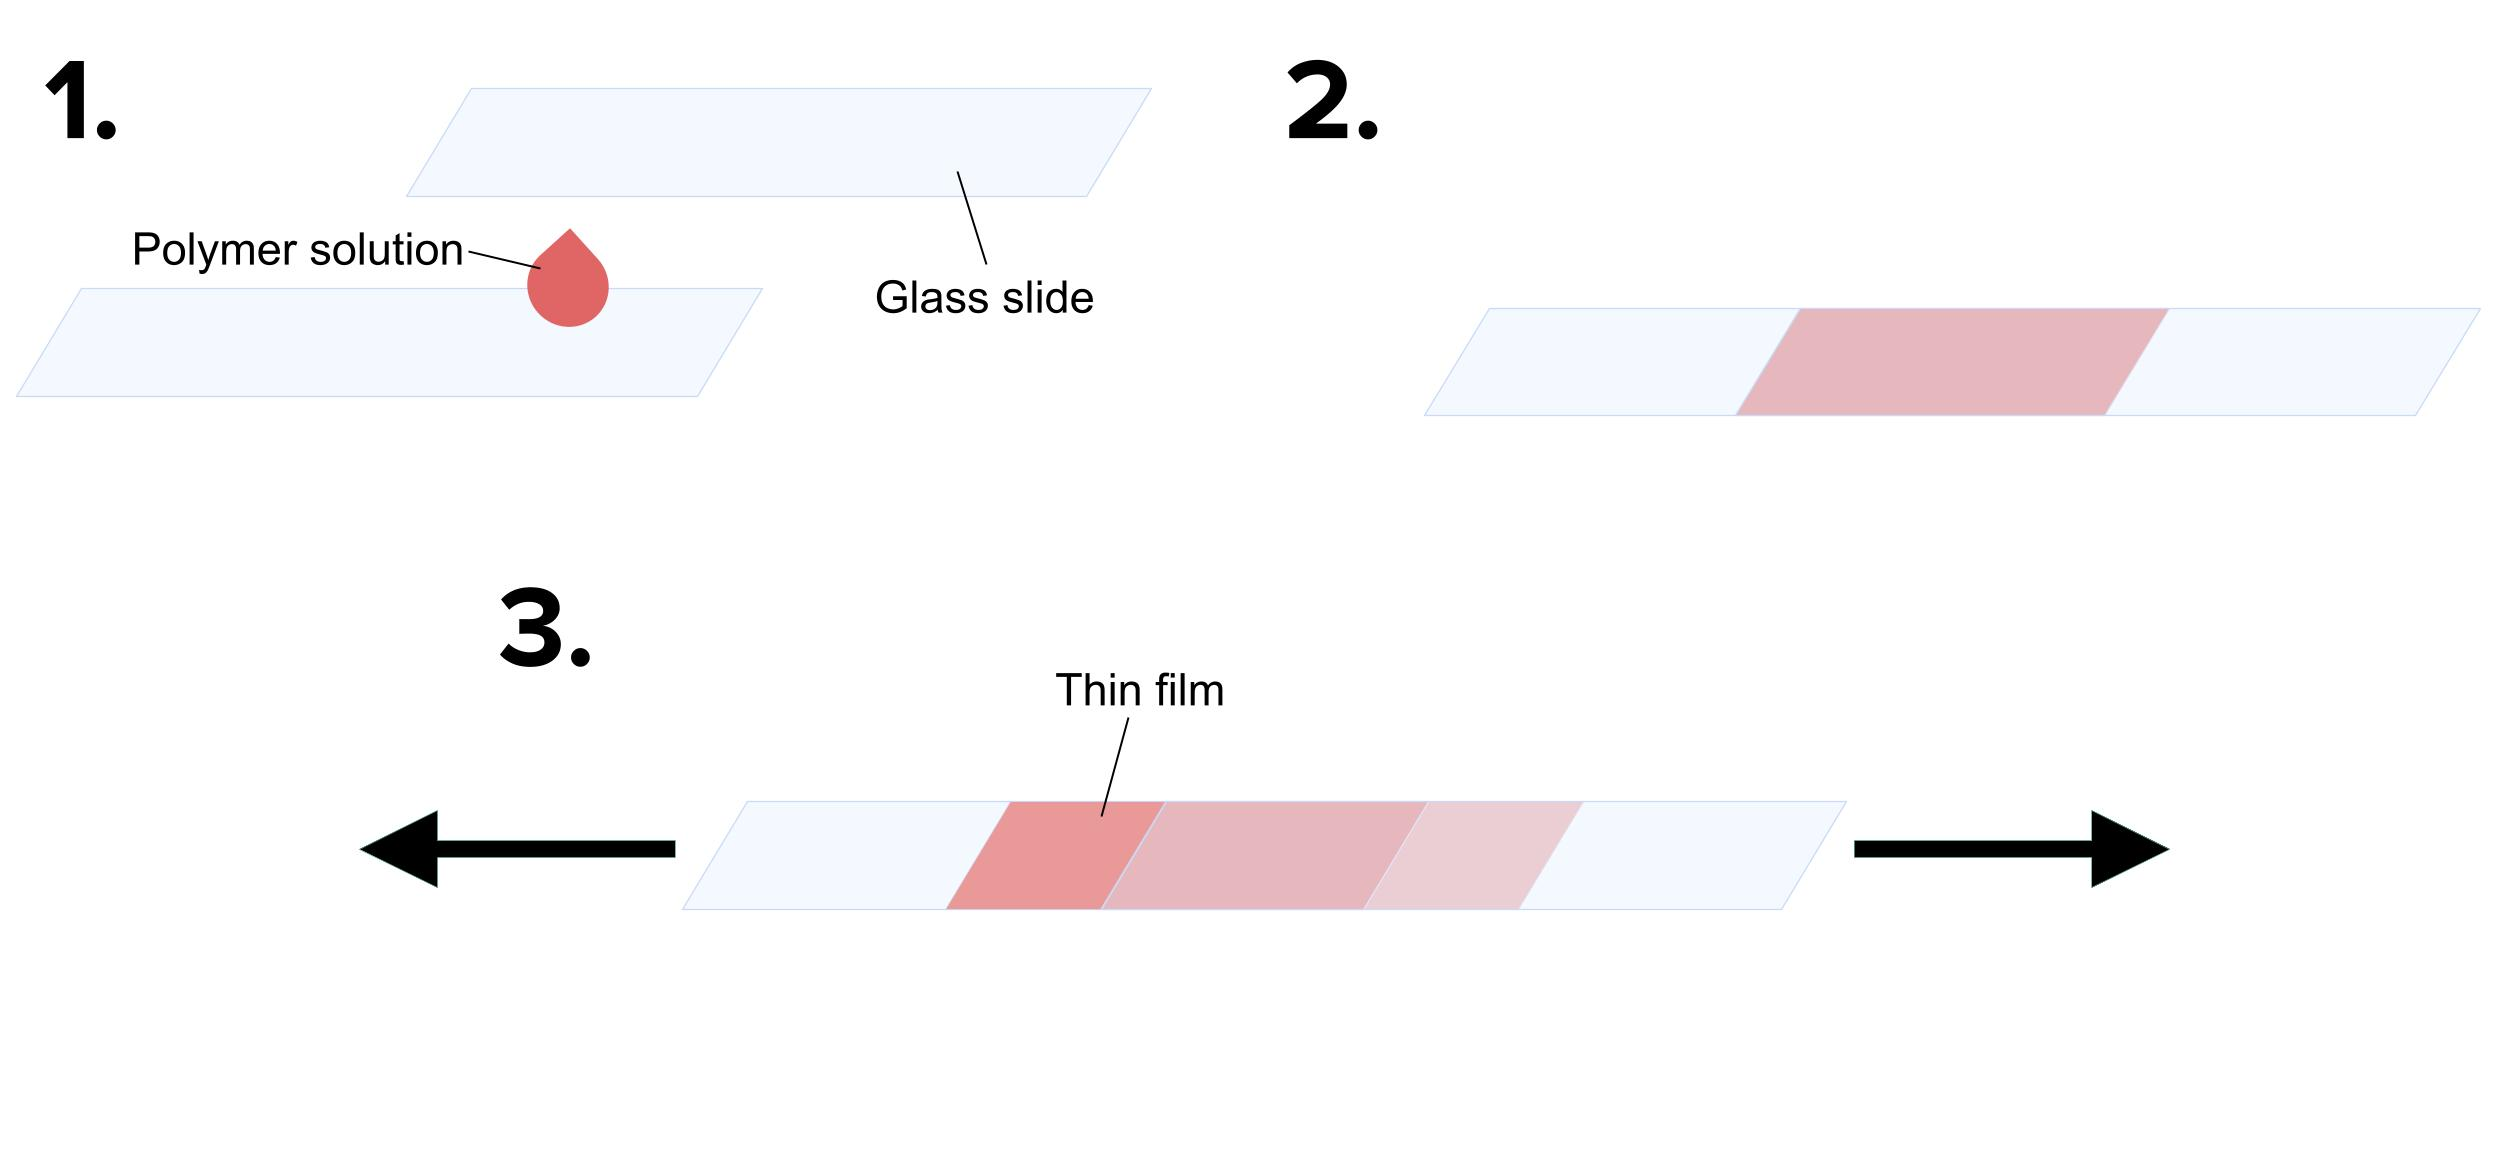
\includegraphics[width = 14cm]{schematic.jpg}
	\caption{Schematic of slip-coating process.}
\end{figure}

\begin{figure}[H]
	\centering
	\captionsetup{width=18cm}
	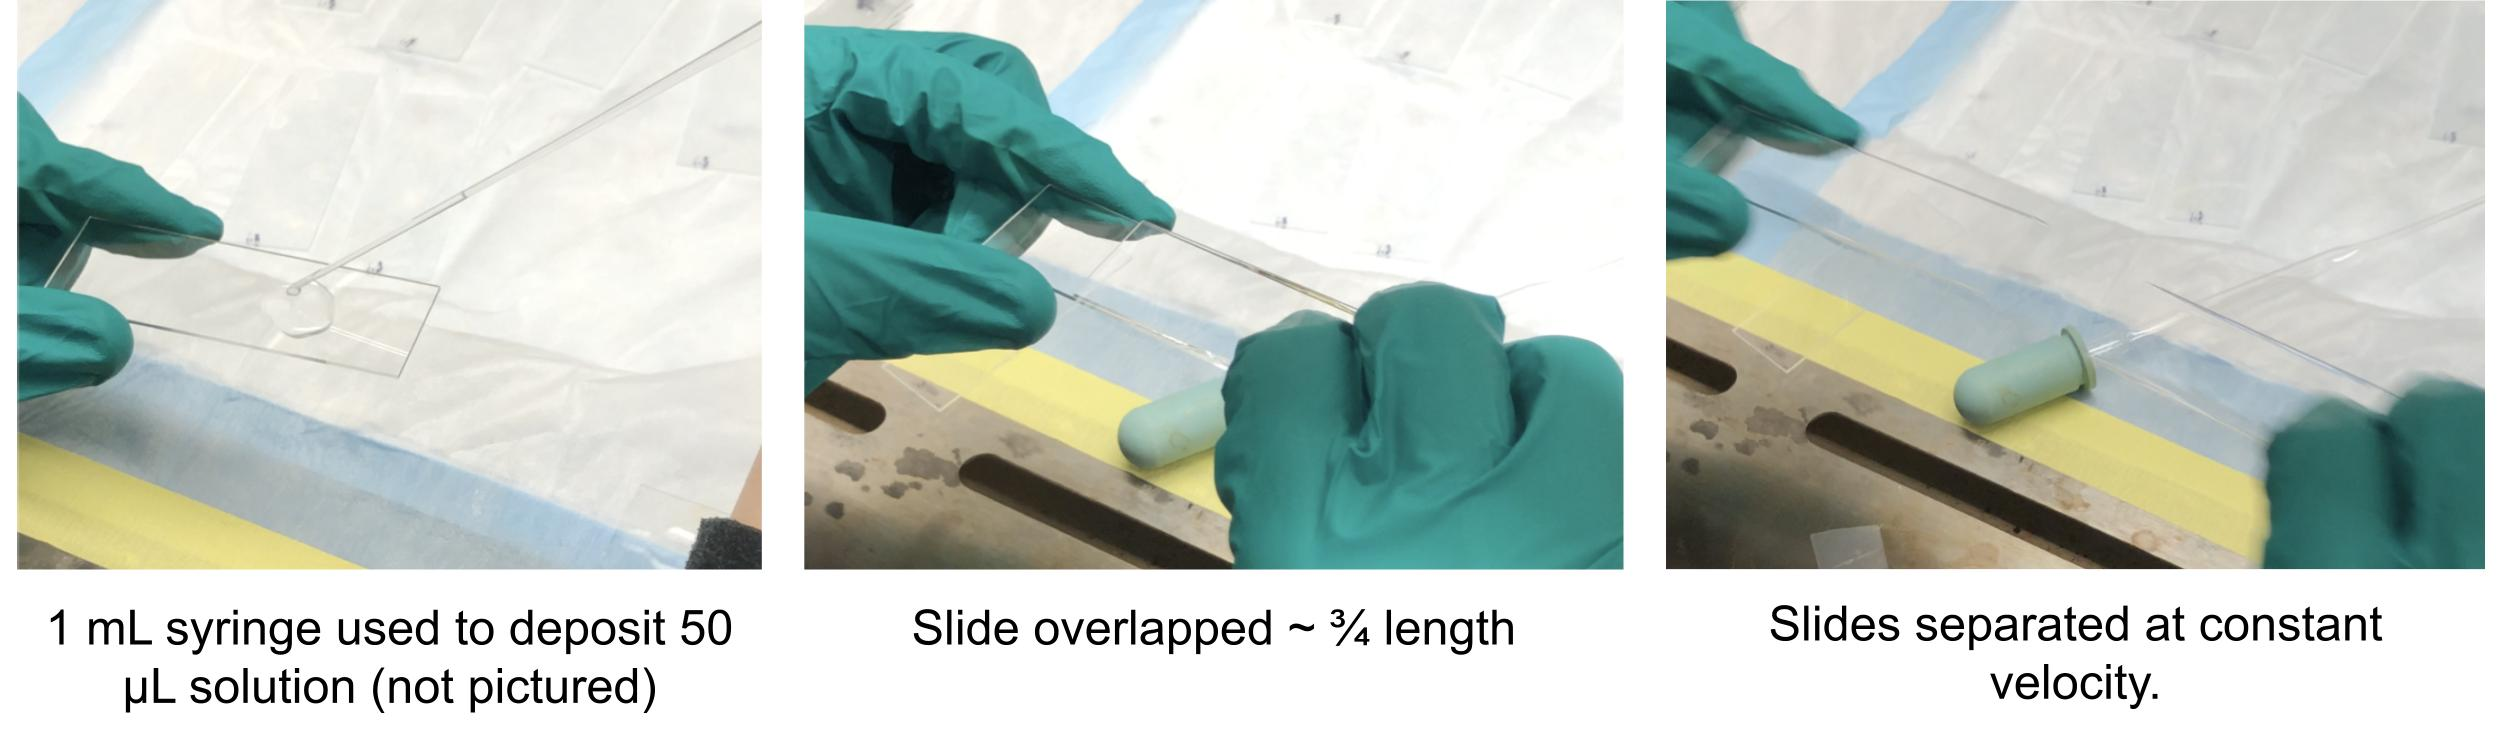
\includegraphics[width = 18cm]{Slip-Coat-Pic.jpg}
	\caption{Procedural images of slip=coating process. Pictured is PVC dissolved into THF and cyclohexane.}
\end{figure}

\begin{figure}[H]
	\centering
	\begin{minipage}{11.5cm}
		\centering
		\captionsetup{width=10cm}
		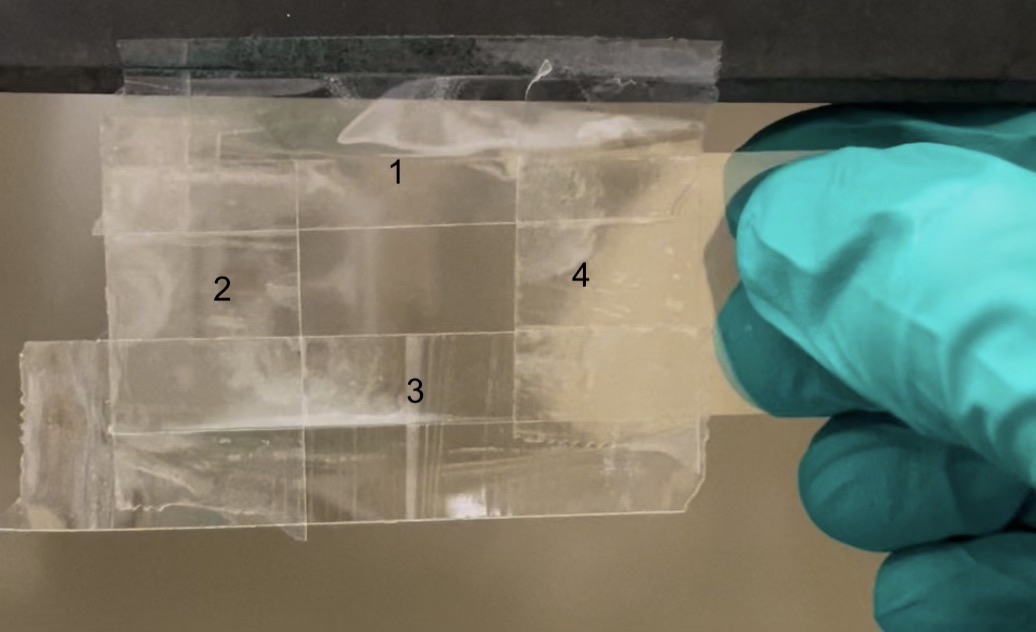
\includegraphics[width = 10cm]{IMG_4446.jpeg}
		\caption{A completed tape frame (on unfrosted tape). The order of application of tapestrips is important, and generally follows a (counter) clockwise direction.}
	\end{minipage}%
	\begin{minipage}{8.5cm}
		\centering
		\captionsetup{width=5cm}
		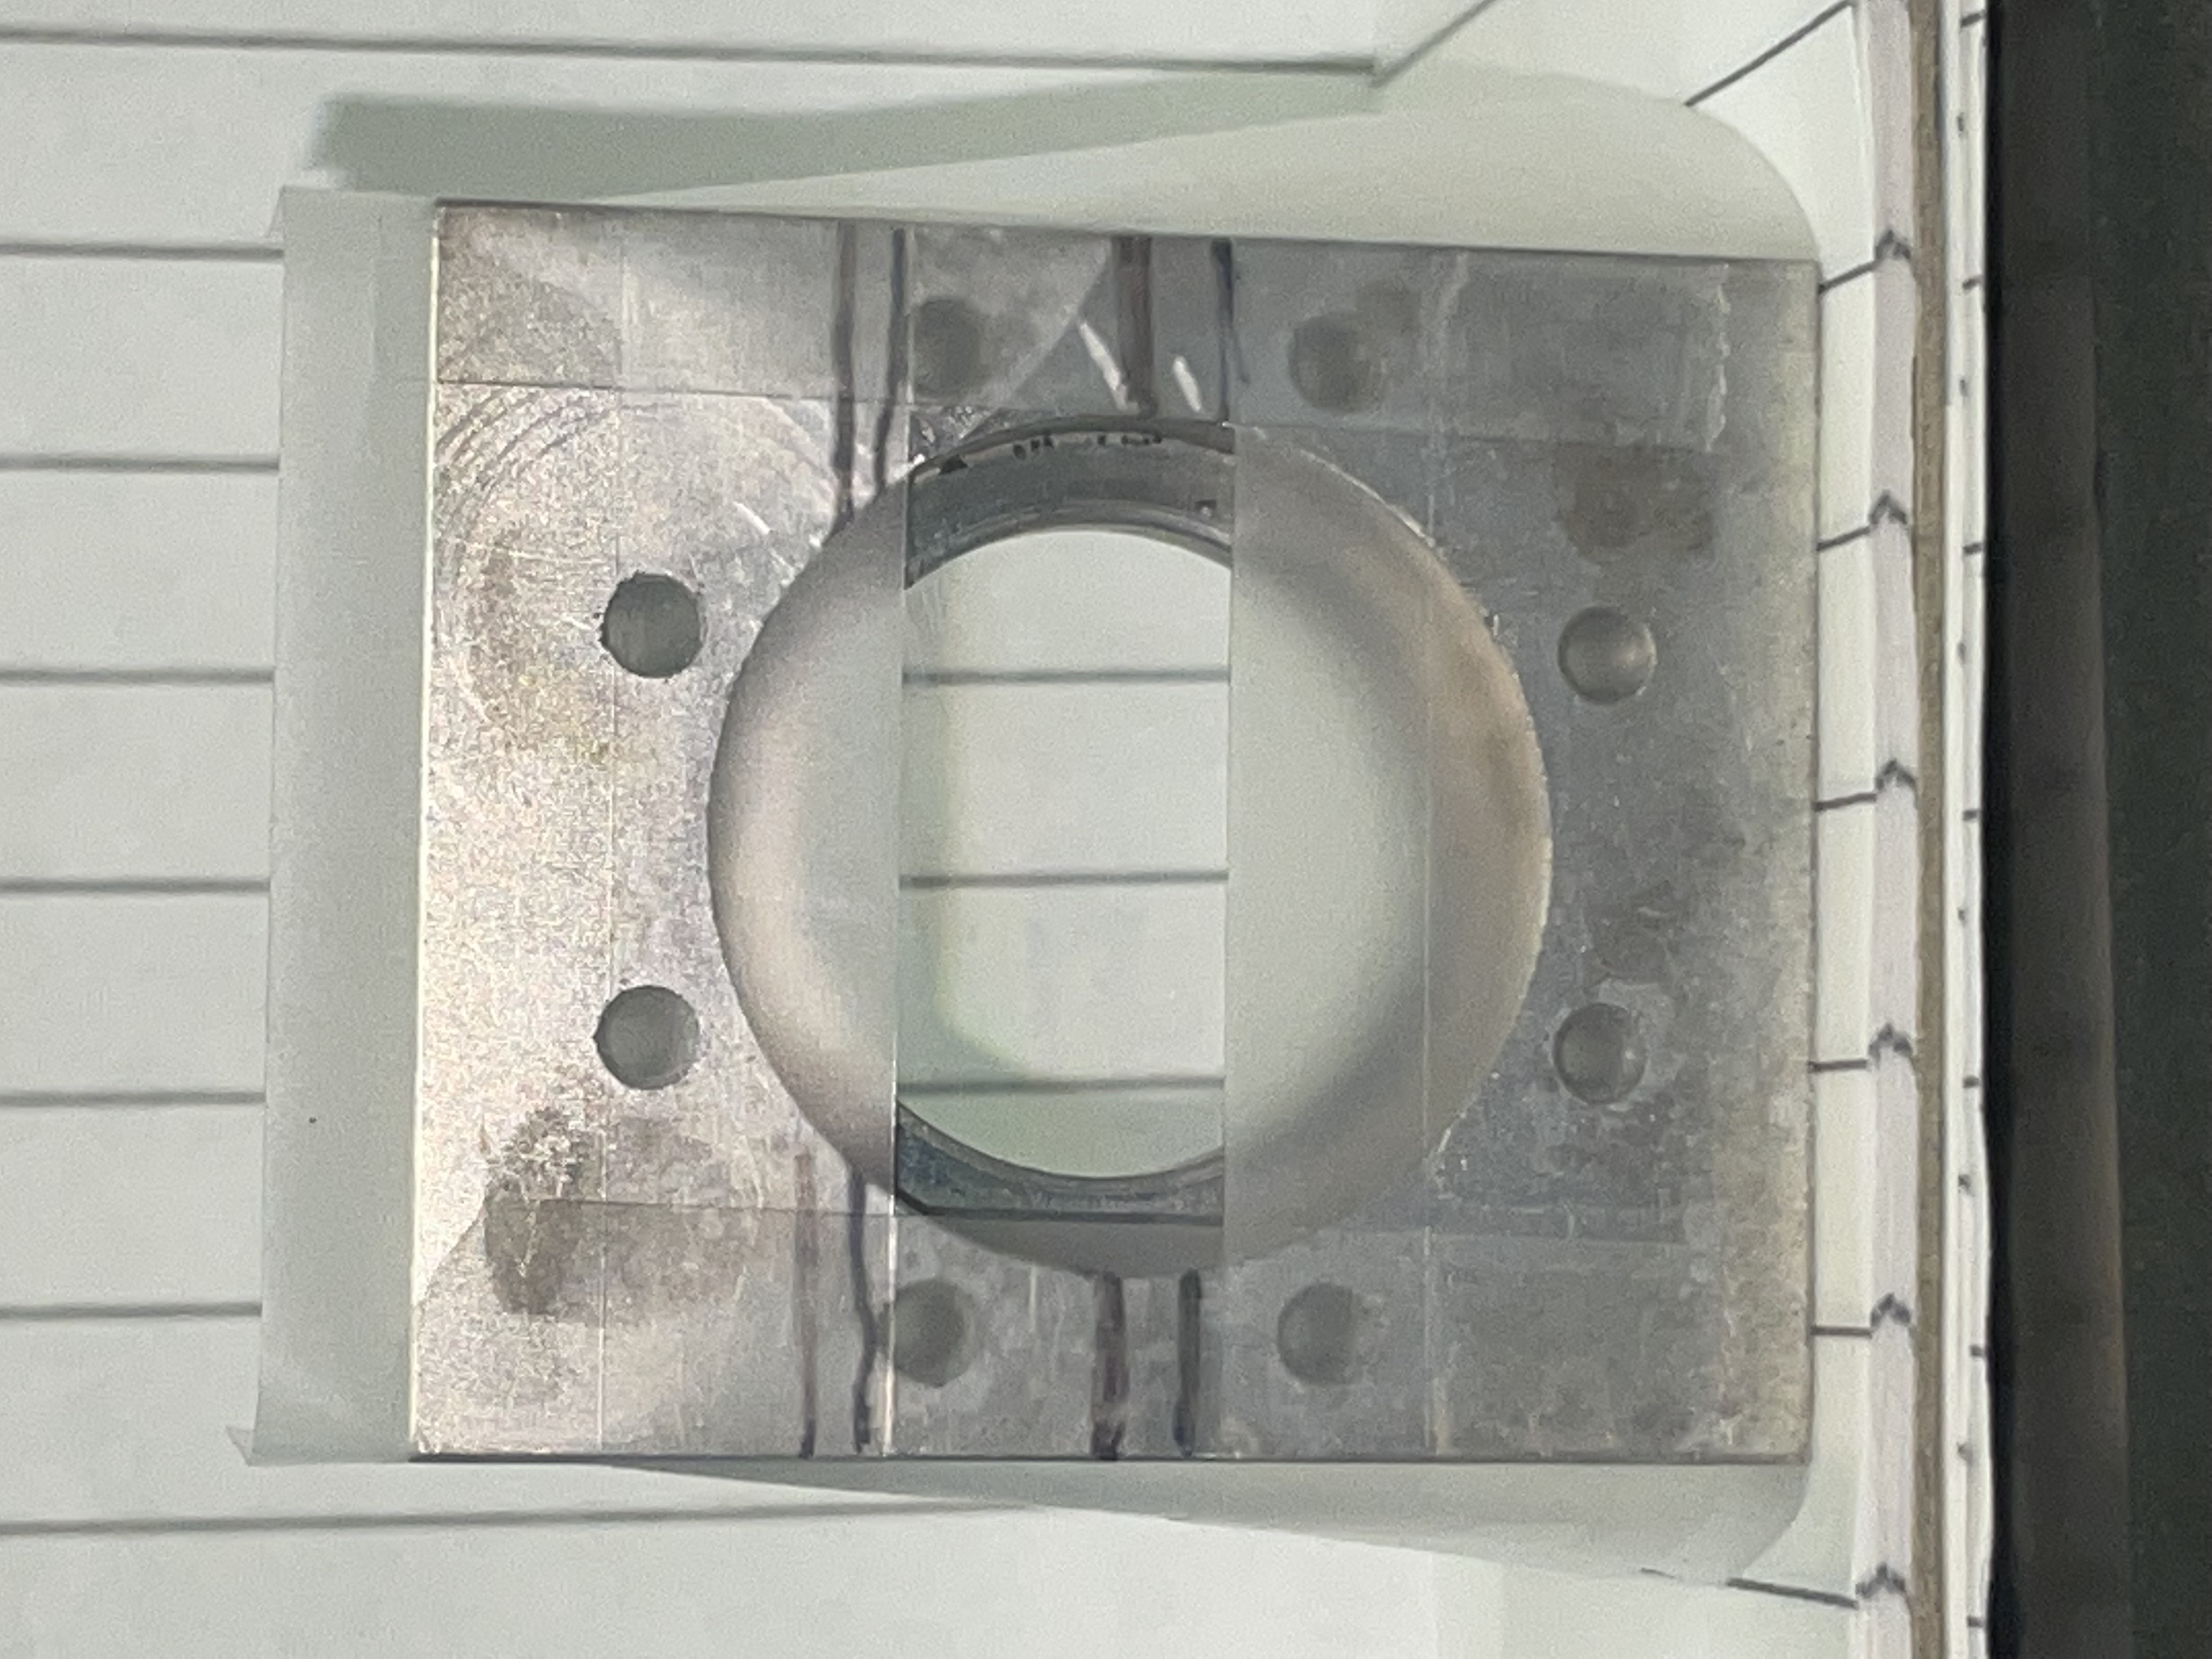
\includegraphics[width = 8cm,angle=270,origin=c]{IMG_4412.jpeg}
		\caption{A successfully delaminated film, now placed onto FTIR mount for UV-vis scan.}
	\end{minipage}
\end{figure}  

\begin{center}
\begin{tabular}{ |p{\textwidth}| }
\hline
\cellcolor{gray!25} \#6 \textbf{Special Handling Procedures and Storage Requirements} \\
\hline
Flammable solvents must be stored within a fire cabinet. Peroxide-forming solvents must be properly stored in an air impermeable container. Carcinogenic solvents are handled only with proper PPE.
\\ \hline
\end{tabular}
\end{center}

\begin{center}
\begin{tabular}{ |p{\textwidth}| }
\hline
\cellcolor{gray!25} \#7 \textbf{Decontamination} \\
\hline
Gloves must be properly disposed of as contaminated waste due to possible exposure to solvents during procedure. 
\\ \hline
\end{tabular}
\end{center}

\begin{center}
\begin{tabular}{ |p{\textwidth}| }
\hline
\cellcolor{gray!25} \#8 \textbf{Emergency Procedures} \\
\hline
\underline{Safety Shower/Eye Shower}: \\
Any serious chemical self-contamination \\
\underline{Evacuate the Lab, and call 911 if}: \\
1. Serious chemical self-contamination \\
2. Large hazardous material release \\
3. Smoke, chemical fire, explosion \\
\underline{Call ext. 5555 if}: \\
1. Non-life threatening injury \\
2. Non-life threatening chemical or radiation incident   
\\ \hline
\end{tabular}
\end{center}

\begin{center}
\begin{tabular}{ |p{\textwidth}| }
\hline
\cellcolor{gray!25} \#9 \textbf{Waste Disposal} \\
\hline
Once to be disposed of, the polymer solutions must be disposed of according to the solvent classification. This procedure can yield 50 mL of liquid waste (10 separate 5 mL vials), depending on how much solution is used. Moreover, syringes and damaged glass slides must be disposed of as sharps. Further disposal is handled by department. 
\\ \hline
\end{tabular}
\end{center}

\begin{center}
\begin{tabular}{ |p{\textwidth}| }
\hline
\cellcolor{gray!25} \#10 \textbf{Training Requirements} \\
\hline
Laboratory Safety Orientation \\
Compressed Gases Training (to extract peroxide forming solvents) \\
Cryogenic Liquids and Oxygen Deficiency Training
\\ \hline
\end{tabular}
\end{center}

\begin{center}
\begin{tabular}{ |p{\textwidth}| }
\hline
\cellcolor{gray!25} \#11 \textbf{Approval Required} \\
\hline
N/A
\\ \hline
\end{tabular}
\end{center}

\end{document}
